
gnuplot is a famous and widely used command-line program that can 
generate two- and three-dimensional plots of functions, data, and data fits.
It dates back to 1986 and runs on all operating systems (Linux, Unix, Microsoft Windows, macOS). 

\url{http://www.gnuplot.info/}

\url{http://www.gnuplotting.org/}

\url{http://lowrank.net/gnuplot/index-e.html}

The gray boxes indicate that its content takes place in the terminal.

%----------------------------------------
\subsection*{Installing gnuplot}

If you are using Ubuntu, you can install gnuplot as follows:


\begin{mdframed}[backgroundcolor=gray!10]
\begin{verbatim}
> sudo apt-get install gnuplot
\end{verbatim}
\end{mdframed}


%----------------------------------------
\subsection*{Interactive use}

In the following pages I explain how to use the gnuplot program from the terminal.
Having done so, in the terminal simply type

\begin{mdframed}[backgroundcolor=gray!10]
\begin{verbatim}
> gnuplot
\end{verbatim}
\end{mdframed}

The following should then appear:

\begin{mdframed}[backgroundcolor=gray!10]
\begin{verbatim}

	G N U P L O T
	Version 5.2 patchlevel 2    last modified 2017-11-01 

	Copyright (C) 1986-1993, 1998, 2004, 2007-2017
	Thomas Williams, Colin Kelley and many others

	gnuplot home:     http://www.gnuplot.info
	faq, bugs, etc:   type "help FAQ"
	immediate help:   type "help"  (plot window: hit 'h')

Terminal type is now 'wxt'

gnuplot>
\end{verbatim}
\end{mdframed}

The prompt means that gnuplot is expecting instructions. We start by making sure that 
the terminal type is such that a window appears in this interactive mode. We test this 
by plotting a simple function, $f(x)=x$:

\begin{mdframed}[backgroundcolor=gray!10]
\begin{verbatim}
gnuplot> plot x
\end{verbatim}
\end{mdframed}


You should then obtain something similar:

\begin{center}
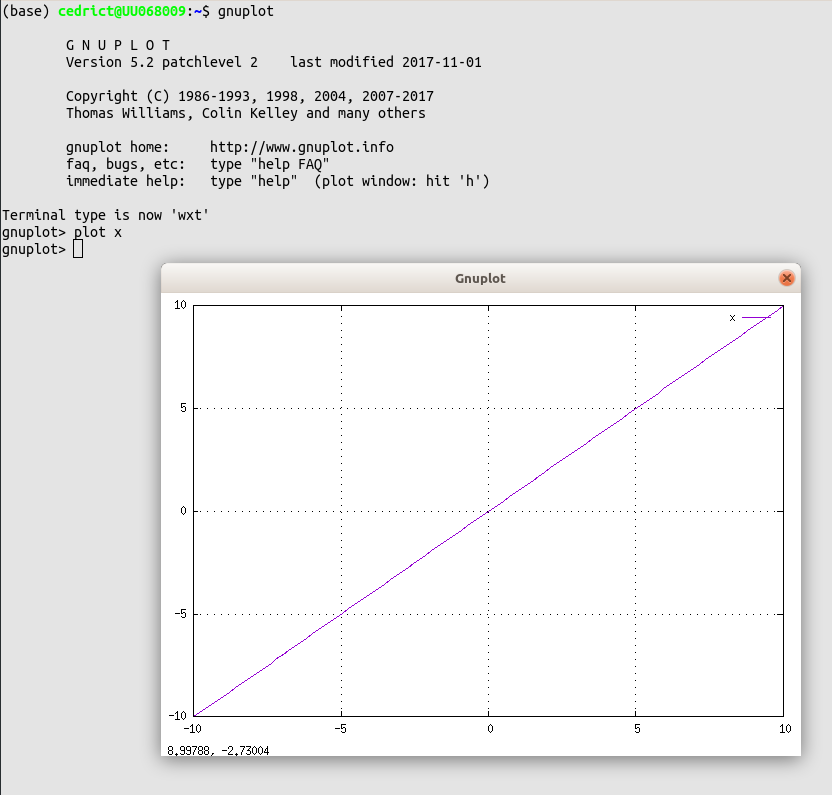
\includegraphics[width=7cm]{images/gnuplot/gnuplot1}
\end{center}

You can specify the $x$ range, change the function to $x^2+\sqrt{x}$ and label the axes as follows:

\begin{mdframed}[backgroundcolor=gray!10]
\begin{verbatim}
gnuplot> set xlabel 'time'
gnuplot> set ylabel 'cost'
gnuplot> plot[-5:7] x**2+sqrt(x)
\end{verbatim}
\end{mdframed}

\begin{center}
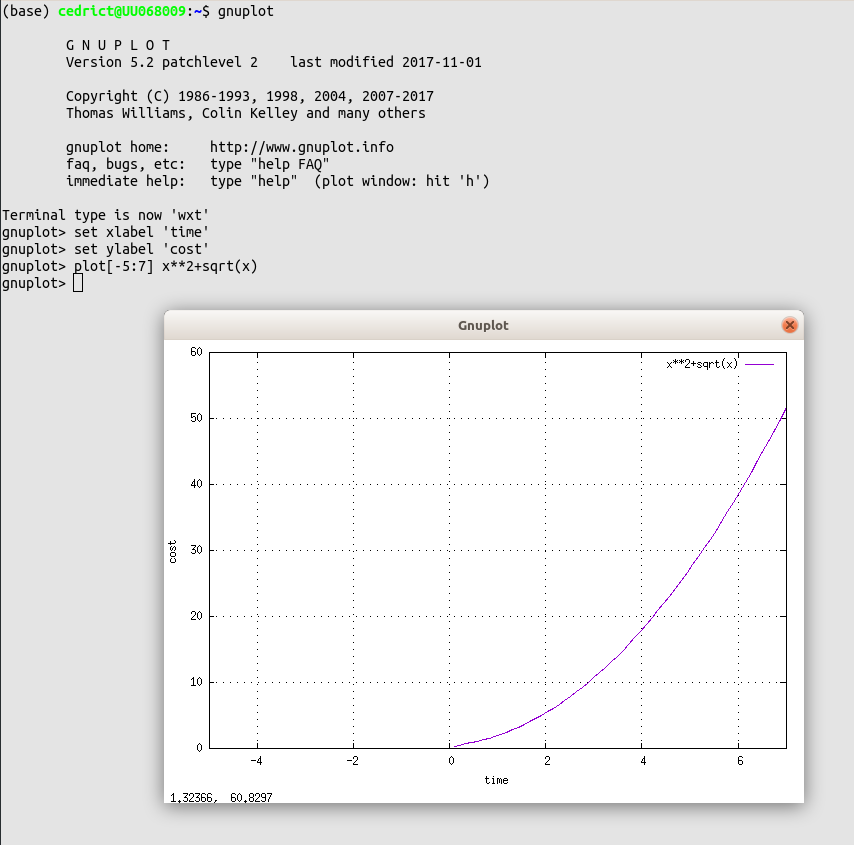
\includegraphics[width=7cm]{images/gnuplot/gnuplot2}
\end{center}
We can also plot functions of both $x$ and $y$ as follows:
\begin{mdframed}[backgroundcolor=gray!10]
\begin{verbatim}
gnuplot> splot x*y, x**2+y
\end{verbatim}
\end{mdframed}
and we get
\begin{center}
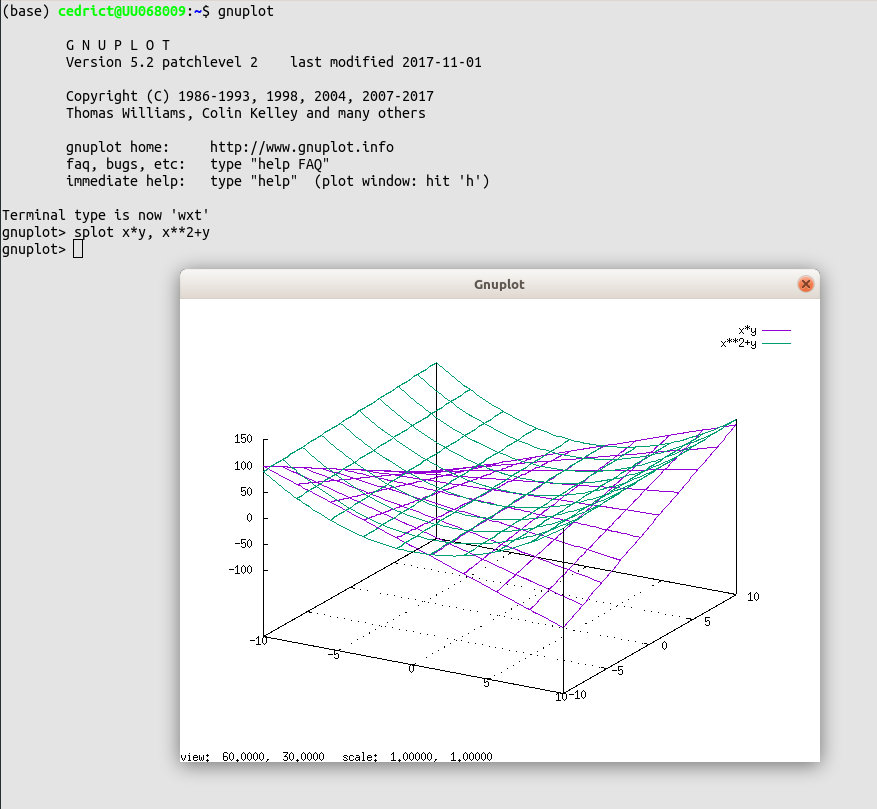
\includegraphics[width=7cm]{images/gnuplot/gnuplot3}
\end{center}

Another nice feature in the interactive is the fact that you can use the left button of the mouse
to rotate the plot! 

Finally, let us assume that there is a file {\filenamefont results.dat} in the folder and that it contains 
results from experimental measurements or numerical values organised in columns as follows:
\begin{verbatim}
 1e17 8 0 256000 384000 4.91094e-12 -0.00533647 -714769 0
 1e17 32 0 256000 384000 1.96438e-11 -0.0213459 -2.85908e+06 0
 1e17 128 0 256000 384000 7.8575e-11 -0.0853835 -1.14363e+07 0
 2e17 8 0 256000 384000 3.43871e-12 -0.00533555 -714753 0
 2e17 32 0 256000 384000 1.37548e-11 -0.0213422 -2.85901e+06 0
 2e17 128 0 256000 384000 5.50193e-11 -0.0853688 -1.1436e+07 0
 4e17 8 0 256000 384000 4.13458e-12 -0.00533372 -714720 0
 ...
 67108864e17 128 0 256000 384000 -5.28841e-12 -0.0212269 -1.27701e+07 0
 134217728e17 8 0 256000 384000 2.93622e-13 -0.00132619 -798163 0
 134217728e17 32 0 256000 384000 1.17449e-12 -0.00530475 -3.19265e+06 0
 134217728e17 128 0 256000 384000 4.69795e-12 -0.021219 -1.27706e+07 0
 268435456e17 8 0 256000 384000 4.03077e-13 -0.00132594 -798181 0
 268435456e17 32 0 256000 384000 1.61231e-12 -0.00530376 -3.19272e+06 0
 268435456e17 128 0 256000 384000 6.44923e-12 -0.0212151 -1.27709e+07 0
\end{verbatim} 
In this case we may with to plot the 6th column as a function of the 1st one:
\begin{mdframed}[backgroundcolor=gray!10]
\begin{verbatim}
plot 'results.dat' using 1:6 with linespoint linewidth 2 title 'velocity'
\end{verbatim}
\end{mdframed}
\begin{center}
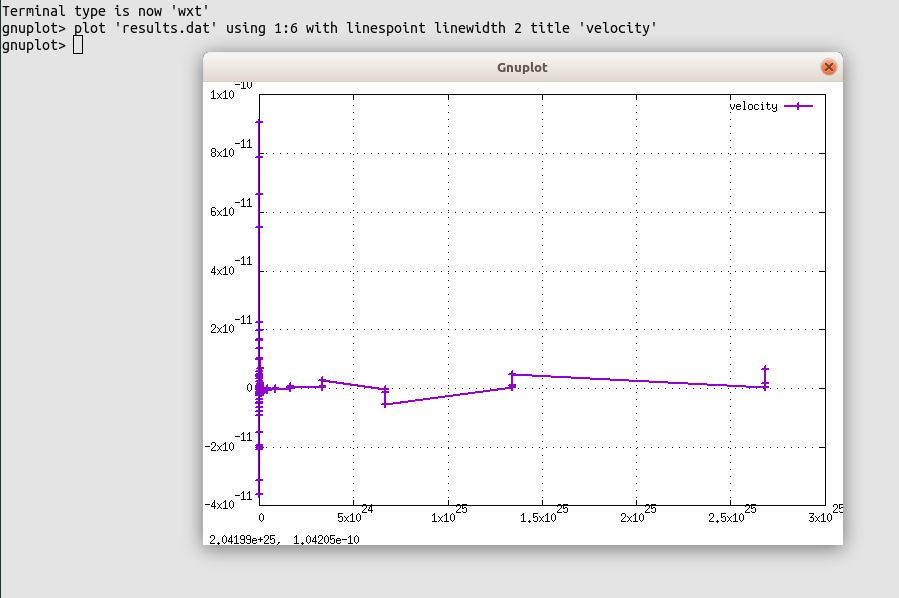
\includegraphics[width=7cm]{images/gnuplot/gnuplot4}
\end{center}
Since typing these instructions time and time again is a bit tedious gnuplot 
allows the user to use short versions of these commands:
\begin{mdframed}[backgroundcolor=gray!10]
\begin{verbatim}
gnuplot> plot 'results.dat' u 1:6 w lp lw 2 t 'velocity'
\end{verbatim}
\end{mdframed}
We see that the range of $x$ values spans many order of magnitudes so we wish to use 
a logarithmic scale on the $x$-axis. 
\begin{mdframed}[backgroundcolor=gray!10]
\begin{verbatim}
gnuplot> set log x
\end{verbatim}
\end{mdframed}
Also, I can combine data with analytical function:
\begin{mdframed}[backgroundcolor=gray!10]
\begin{verbatim}
gnuplot> set log x
gnuplot> plot 'results.dat' u 1:6 w lp lw 2 t 'velocity', 1e7/x lw 3 , 6e-11 
\end{verbatim}
\end{mdframed}

\begin{center}
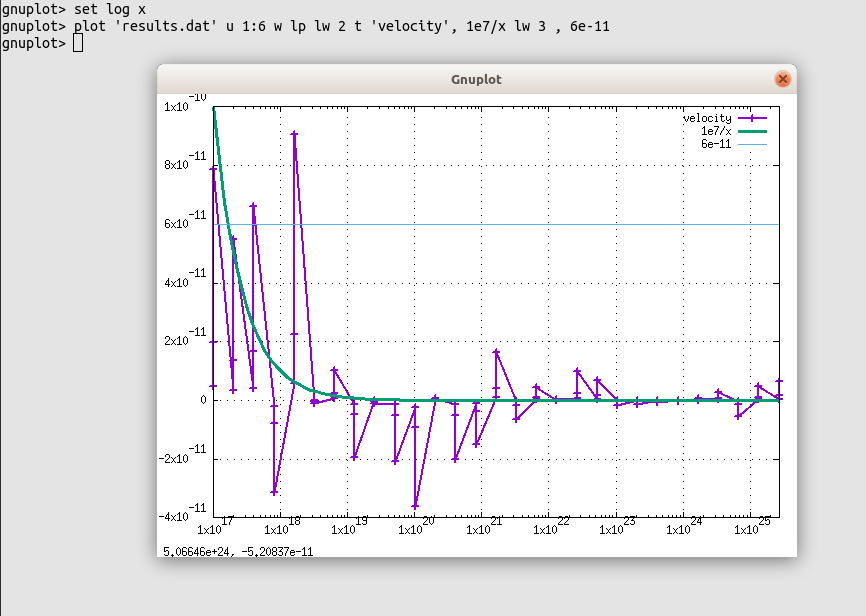
\includegraphics[width=7cm]{images/gnuplot/gnuplot5}
\end{center}
Finally, we may wish to export the plot to a file, say a pdf file. We must then 
re-assign the terminal, give a name to the file and re-plot:
\begin{mdframed}[backgroundcolor=gray!10]
\begin{verbatim}
gnuplot> set term pdf
gnuplot> set output 'results.pdf'
gnuplot> plot 'results.dat' u 1:6 w lp lw 2 t 'velocity', 1e7/x lw 3 , 6e-11 
\end{verbatim}
\end{mdframed}
You can exit the session by typing
\begin{mdframed}[backgroundcolor=gray!10]
\begin{verbatim}
gnuplot> exit 
\end{verbatim}
\end{mdframed}
You should find {\filenamefont results.pdf} in your folder next to {\filenamefont results.dat}.

%----------------------------------------
\subsection*{Scripting gnuplot}

Although the interactive approach is very useful its workflow 
is not practical if one wishes (for instance) to produce the same plot 
with different data, or to communicate a figure to another scientist. 

We will therefore now turn to scripting. The idea is simple: 
write all the gnuplot commands in a text file, say {\filenamefont script.gnuplot} 
and pass this script as argument to gnuplot:
\begin{mdframed}[backgroundcolor=gray!10]
\begin{verbatim}
> gnuplot script.gnuplot 
\end{verbatim}
\end{mdframed}
This file contains the following:
\begin{verbatim}
set term pdf font "Times,12pt"
set output 'results.pdf'
set grid
set xlabel 'x'
set ylabel 'cost'
set log x
set title 'my title above the plot'
plot 'results.dat' u 1:6 w lp lw 2 t 'velocity', 1e7/x lw 3 t 'fit' , 6e-11 t 'threshold'
\end{verbatim}

\begin{center}
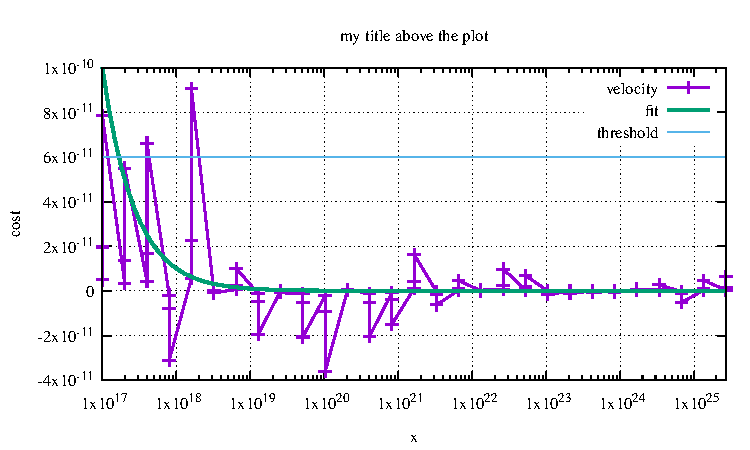
\includegraphics[width=7cm]{images/gnuplot/results.pdf}
\end{center}
Note that I have added a title to the plot as well. 




%----------------------------------------
\subsection*{How to}


%----------------------------------------
\subsubsection*{Greek letters}

In order to display Greek letters the {\tt /Symbol} command:

\begin{verbatim}
set xlabel '{/Symbol d}{/Symbol r}' 
\end{verbatim}

\begin{tabular}{ll|ll|ll|ll}
\hline
Alphabet&Symbol  &Alphabet 	&Symbol   &Alphabet 	&Symbol  &Alphabet 	&Symbol  \\
\hline
\hline
A 	&Alpha 	 &N 		&Nu 	  &a 		&alpha ($\alpha$)     &n 		&nu  $\nu$\\
B 	&Beta 	 &O 		&Omicron  &b 		&beta  ($\beta$)      &o 		&omicron  \\
C 	&Chi 	 &P 		&Pi 	  &c 		&chi   ($\chi$)	      &p 		&pi  $\pi$\\
D 	&Delta 	 &Q 		&Theta 	  &d 		&delta  ($\delta$)    &q 		&theta $\theta$ \\
E 	&Epsilon &R 		&Rho 	  &e 		&epsilon ($\epsilon$) &r 		&rho  $\rho$\\
F 	&Phi 	 &S 		&Sigma 	  &f 		&phi 	($\phi$)      &s 		&sigma  $\sigma$\\
G 	&Gamma 	 &T 		&Tau 	  &g 		&gamma 	($\gamma$)    &t 		&tau  $\tau$\\
H 	&Eta 	 &U 		&Upsilon  &h 		&eta 	($\eta$)      &u 		&upsilon  $\upsilon$\\
I 	&iota 	 &W 		&Omega 	  &i 		&iota 	($\iota$)     &w 		&omega  $\omega$\\
K 	&Kappa 	 &X 		&Xi 	  &k 		&kappa 	($\kappa$)    &x 		&xi  $\xi$\\
L 	&Lambda  &Y 		&Psi 	  &l 		&lambda  ($\lambda$)  &y 		&psi  $\psi$\\
M 	&Mu 	 &Z 		&Zeta 	  &m 		&mu 	($\mu$)       &z 		&zeta $\zeta$\\
\hline
\end{tabular}





%----------------------------------------
\subsubsection*{linetype and dashtype}

There are essentially three ways of plotting data: 
\begin{verbatim}
plot 'results.dat' u 1:6 w l 
plot 'results.dat' u 1:6 w p
plot 'results.dat' u 1:6 w lp
\end{verbatim}
corresponding to (from left to right):
\begin{center}
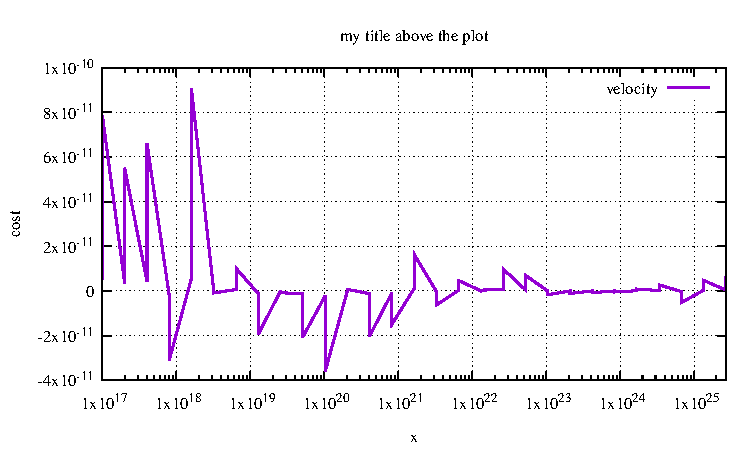
\includegraphics[width=5cm]{images/gnuplot/results_a.pdf}
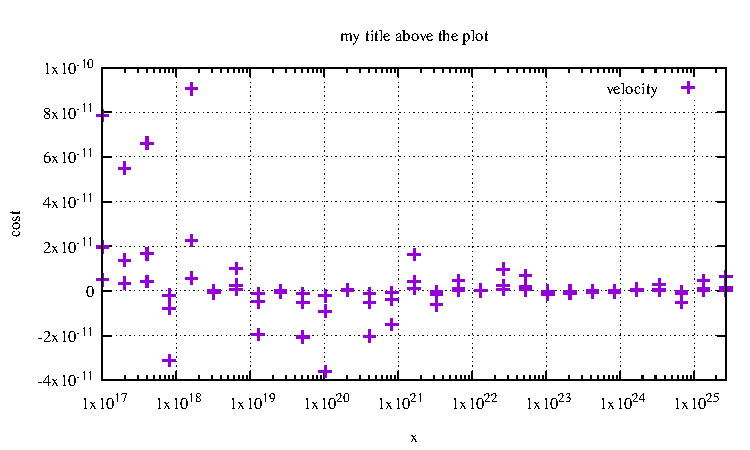
\includegraphics[width=5cm]{images/gnuplot/results_b.pdf}
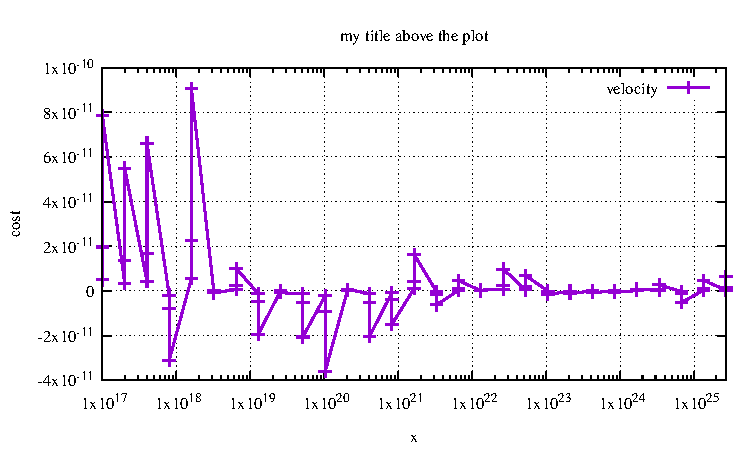
\includegraphics[width=5cm]{images/gnuplot/results_c.pdf}
\end{center}

The following script
\begin{verbatim}
set output 'linetypes.pdf'
plot[][]\
x+0  w l lt 0 t 'linetype 1',\
x+1  w l lt 1 t 'linetype 2',\
x+2  w l lt 2 t 'linetype 3',\
x+3  w l lt 3 t 'linetype 4',\
x+4  w l lt 4 t 'linetype 5',\
x+5  w l lt 5 t 'linetype 6',\
x+6  w l lt 6 t 'linetype 7',\
x+7  w l lt 7 t 'linetype 8',\
x+8  w l lt 8 t 'linetype 9',\
x+9  w l lt 9 t 'linetype 10',\
x+10 w l lt 10 t 'linetype 11',\
x+11 w l lt 11 t 'linetype 12'
\end{verbatim}
generates the following plot:
\begin{center}
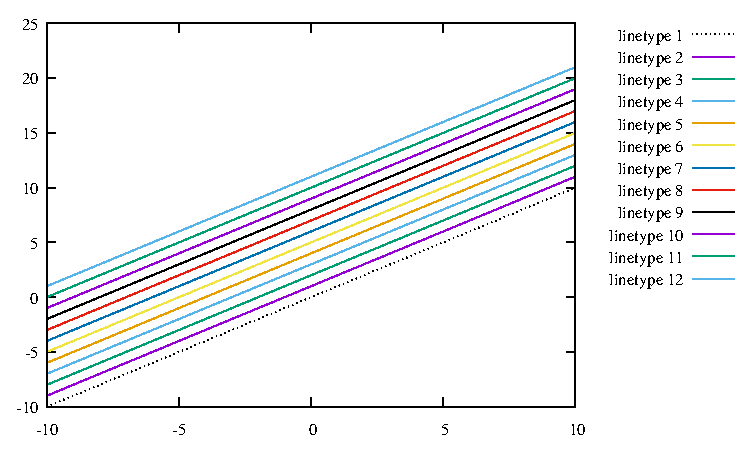
\includegraphics[width=7cm]{images/gnuplot/linetypes.pdf}
\end{center}
We see that the colours repeat from linetype 10. 
Fortunately we can also combine linetypes with dashtypes.
The following script
\begin{verbatim}
set output 'dashtypes.pdf'
plot[][]\
x+1  w l lt 1  dt 1 t 'linetype 2',\
x+2  w l lt 2  dt 2 t 'linetype 3',\
x+3  w l lt 3  dt 3 t 'linetype 4',\
x+4  w l lt 4  dt 4 t 'linetype 5',\
x+5  w l lt 5  dt 5 t 'linetype 6',\
x+6  w l lt 6  dt 6 t 'linetype 7',\
x+7  w l lt 7  dt 7 t 'linetype 8',\
x+8  w l lt 8  dt 8 t 'linetype 9',\
x+9  w l lt 9  dt 9 t 'linetype 10',\
x+10 w l lt 10 dt 10 t 'linetype 11',\
x+11 w l lt 11 dt 11 t 'linetype 12' 
\end{verbatim}
generates the following plot
\begin{center}
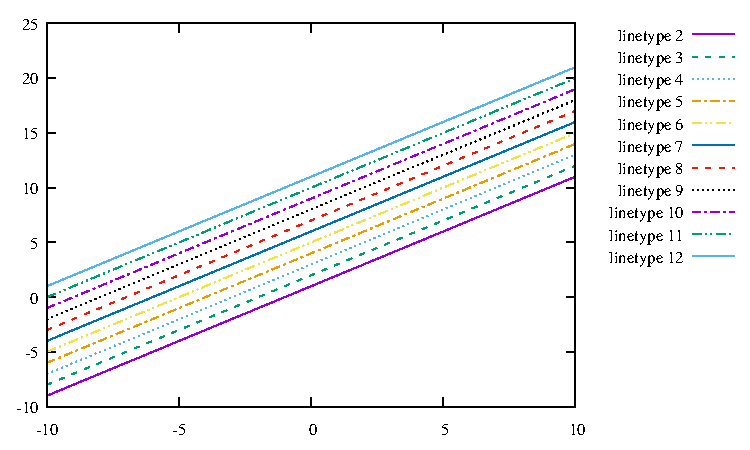
\includegraphics[width=7cm]{images/gnuplot/dashtypes.pdf}
\end{center}
and we see that there are only 5 different dash types. 

Finally, we turn to point types.
The following script
\begin{verbatim}
set output 'pointtypes.pdf'
plot[][]\
x+0  w p pt 0  ps .5 t 'linetype 1',\
x+1  w p pt 1  ps .5 t 'linetype 2',\
x+2  w p pt 2  ps .5 t 'linetype 3',\
x+3  w p pt 3  ps .5 t 'linetype 4',\
x+4  w p pt 4  ps .5 t 'linetype 5',\
x+5  w p pt 5  ps .5 t 'linetype 6',\
x+6  w p pt 6  ps .5 t 'linetype 7',\
x+7  w p pt 7  ps .5 t 'linetype 8',\
x+8  w p pt 8  ps .5 t 'linetype 9',\
x+10 w p pt 10 ps .5 t 'pointtype 10',\
x+11 w p pt 11 ps .5 t 'pointtype 11',\
x+12 w p pt 12 ps .5 t 'pointtype 12',\
x+13 w p pt 12 ps .5 t 'pointtype 13',\
x+14 w p pt 12 ps .5 t 'pointtype 14' 
\end{verbatim}
generates the following plot
\begin{center}
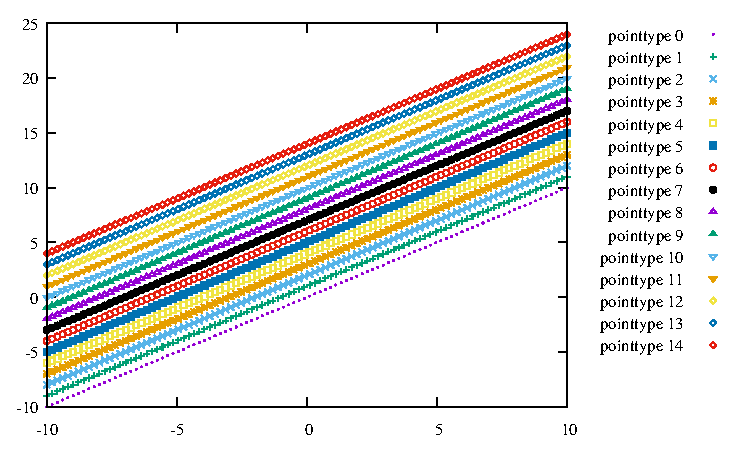
\includegraphics[width=7cm]{images/gnuplot/pointtypes.pdf}
\end{center}
Note that I have used the {\tt ps} command ('point size') to make the points 50\% smaller 
than normal. 


%----------------------------------------
\subsubsection*{Moving the 'key'}

The default is inside top right, but it can be changed, e.g.:
\begin{verbatim}
set key outside
set key bottom left
\end{verbatim}
corresponding to (from left to right):
\begin{center}
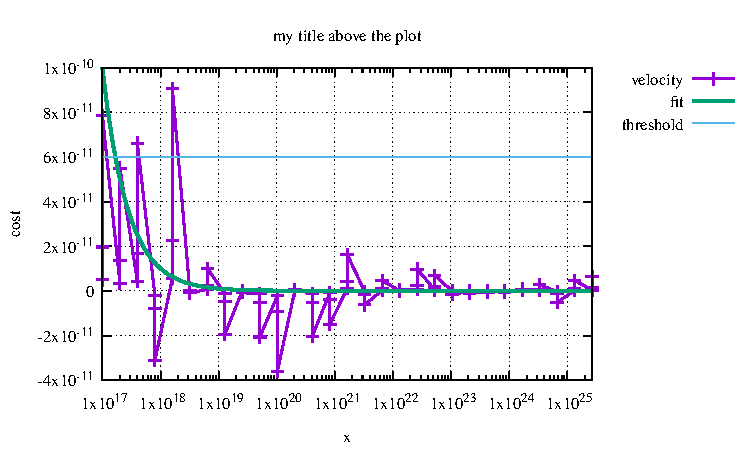
\includegraphics[width=6cm]{images/gnuplot/results_d.pdf}
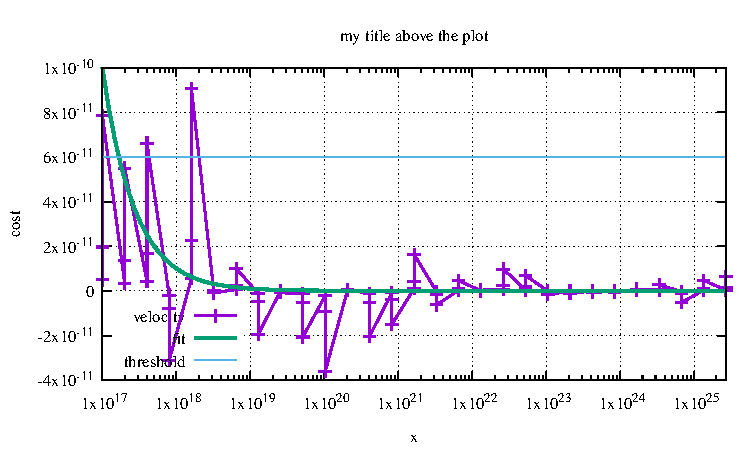
\includegraphics[width=6cm]{images/gnuplot/results_e.pdf}
\end{center}

%----------------------------------------
\subsubsection*{Plotting arrows}

Let us now turn to the {\filenamefont velocity.dat} file which consists of 
four columns: x, y, $\upnu_x$ and $\upnu_y$.

\begin{verbatim}
set output 'velocity_1.pdf'
set xlabel 'x' 
set ylabel 'y' 
set xtics 0.125
set ytics 0.333333333333
set grid
set size square
plot[0:1][0:1]\
'velocity.dat' u 1:2:3:4 w vectors lt -1 notitle 
\end{verbatim}
Note that I have required the plot to be square, that the tics on the 
$x$-axis should be spaced 0.125 while the tics on the $y$-axis should be 
spaced 0.333. 
We obtain the left plot a): 

\begin{center}
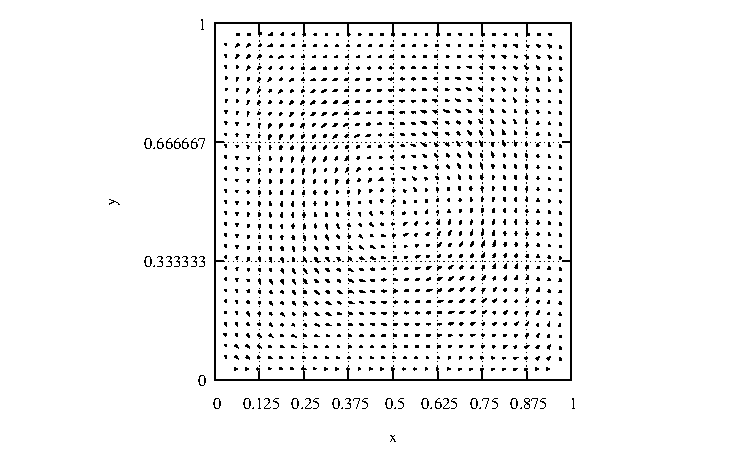
\includegraphics[width=8cm]{images/gnuplot/velocity_1.pdf}
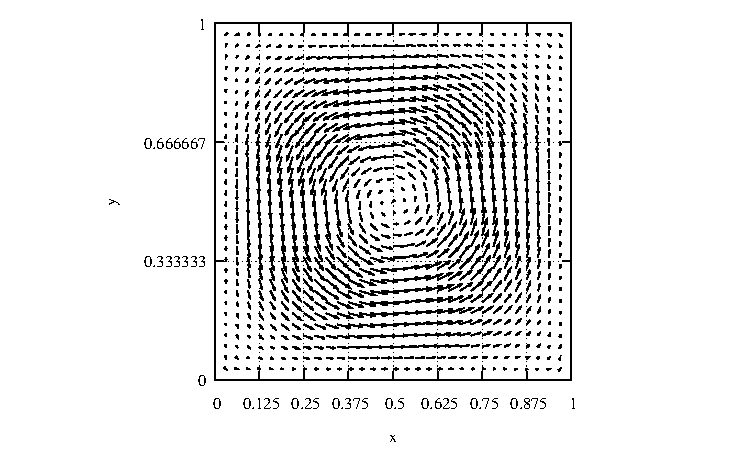
\includegraphics[width=8cm]{images/gnuplot/velocity_2.pdf}
\end{center}

The arrows are too small, so we scale each vector component by a factor 4.
All we need to do is as follows:

\begin{verbatim}
plot[0:1][0:1]\
'velocity.dat' u 1:2:($3*4):($4*4) w vectors lt -1 notitle
\end{verbatim}

Note the dollar sign which 
means that gnuplot takes the value in column 3 or 4 and multiplies it by 4.
The resulting figure is shown in b).




%----------------------------------------
\subsubsection*{Least square fit}


%----------------------------------------
\subsubsection*{coloring areas}


%----------------------------------------
\subsubsection*{vertical line}
